\section{Introduction}\label{sec:introduction}

Finding Steiner trees and related network design problems were intensively studied in undirected graphs, directed graphs, and planar graphs, from the viewpoint of approximation and parameterized algorithms \cite{ChitnisFHM20,eiben_et_al,DBLP:conf/stacs/DvorakFKMTV18,rajesh-andreas-pasin,khandekar,FeldmannM16,DBLP:journals/iandc/BermanBMRY13,DBLP:journals/siamdm/GuoNS11,feldman-ruhl,DBLP:journals/jal/CharikarCCDGGL99,winter1987steiner,hakimi,DBLP:journals/jacm/BateniHM11,DBLP:conf/soda/BateniCEHKM11,DBLP:conf/focs/MarxPP18,karp1972reducibility,ramanathan1996multicast,salama1997evaluation,Li1992267,Natu1997207,daniel-grid-tiling,levin}. The simplest problem of this type is \textsc{Steiner Tree}, where given a graph $G$ and set $T\subseteq V(G)$ of terminals, the task is to find a tree with smallest number of edges that contains every terminal. This problem models a network-design scenario where the terminals need to be connected to each other with a network of minimum cost. \textsc{Steiner Forest} is the generalization where we do not require connection between every pair of terminals, but have to satisfy a given set of demands. Formally, the input of \textsc{Steiner Forest} is a graph $G$ with pairs of vertices $(s_1,t_1)$, $\dots$, $(s_d,t_d)$, the task is to find a subgraph with the minimum number of edges that satisfies every request, that is, $s_i$ and $t_i$ are in the same component of the solution for every $i\in [d]$. 

On directed graphs, \textsc{Directed Steiner Tree (DST)} is defined by specifying one of the terminals in $T$ to be the root and the task is to find a subgraph with the smallest number of edges such that there is path from the root to every terminal in the solution. This problem models a scenario where we need to construct a network where the root can broadcast to every other terminal. An equally natural network design problem on directed graphs is the \textsc{Strongly Connected Steiner Subgraph (SCSS)} problem, where given a directed graph $G$ and a set $T\subseteq V(G)$ of terminals, the task is to find a subgraph with the smallest number of edges where $T$ is in a single strongly connected component, or in other words, the solution contains a path from every terminal to every other terminal. The directed variant of \textsc{Steiner Forest} generalizes both of these problems: in \textsc{Directed Steiner Network (DSN)}, the
input is a digraph $G$ with pairs of vertices $(s_1,t_1)$, $\dots$, $(s_d,t_d)$, and the task is to find a subgraph with the minimum number of edges that has an $s_i\to t_i$ path for every $i\in [d]$.

\paragraph{Planar graphs.} A well-known phenomenon on planar graphs is that the running time of parameterized algorithms for typical NP-hard problems have exponential dependence on $O(\sqrt{k})$, where $k$ is the parameter, and this dependence is best possible assuming the Exponential-Time Hypothesis (ETH)
\cite{DBLP:conf/focs/MarxPP18,ChitnisFHM20,DBLP:conf/focs/FominLMPPS16,DBLP:journals/talg/MarxP22,DBLP:conf/soda/KleinM14,DBLP:conf/icalp/KleinM12,DBLP:conf/icalp/Marx12,DBLP:conf/fsttcs/LokshtanovSW12,DBLP:journals/algorithmica/Verdiere17,DBLP:conf/stoc/Nederlof20a,10.5555/2815661}. All three of \textsc{Directed Steiner Tree},  \textsc{Strongly Connected Steiner Subgraph}, 
and \textsc{Directed Steiner Network} remain NP-hard on planar graphs. However, they behave very differently from the viewpoint of parameterized complexity: the dependence of the running time on the number $k$ of terminals is very different.
\medskip

\mdfdefinestyle{highlight}{frametitlebackgroundcolor=gray!40,backgroundcolor=gray!20,roundcorner=10pt}
\begin{mdframed}[style=highlight,frametitle={Our starting point}] 
     
    \begin{enumerate}    
\item \textsc{Planar DST} can be solved in time $2^k\cdot n^{O(1)}$ \cite{DBLP:conf/stoc/BjorklundHKK07}, but cannot be solved in time $2^{o(k)}\cdot n^{O(1)}$ \cite{DBLP:conf/focs/MarxPP18}, assuming the ETH.
\item \textsc{Planar SCSS} can be solved in time $2^{O(k\log k)}\cdot n^{O(\sqrt{k})}$ \cite{ChitnisFHM20}, but has no algorithm with running time $f(k) \cdot n^{o(\sqrt{k})}$ for any function $f$, assuming the ETH \cite{ChitnisFHM20}.
\item \textsc{Planar DSN} can be solved in time $f(k) \cdot n^{O({k})}$ \cite{eiben_et_al}, but has no algorithm with running time $f(k) \cdot n^{o({k})}$ for any function $f$, assuming the ETH \cite{ChitnisFHM20}.
\end{enumerate}
\end{mdframed}
\medskip

The goal of this paper is to put these results into the context of a wider landscape of directed network design problems. We systematically explore other special cases of  \textsc{Directed Steiner Network} and determine their behavior on planar graphs. Our main result is showing that every special case behaves similarly to one of these three problems: assuming ETH, the best possible running time is of the form $2^{O(k)}\cdot n^{O(1)}$, $f(k) \cdot n^{O(\sqrt{k})}$, or $f(k)\cdot n^{O(k)}$. Furthermore, we provide an exact combinatorial characterization of the problems belonging to the three classes.
\clearpage

\paragraph{Dichotomy for general graphs.}
We explore the different special cases of \textsc{Directed Steiner Network} on planar graphs in a framework similar to how Feldmann and Marx~\cite{FeldmannM16} treated the problem on general graphs. We can define various special cases of \textsc{Directed Steiner Network} by looking at what kind of graph the connection demands define on the terminals: it is an out-star for \textsc{Directed Steiner Tree}, a bidirected clique for \textsc{Strongly Connected Steiner Subgraph}, and a matching for \textsc{Directed Steiner Network}. More generally, for every class $\calD$ of directed graphs, we investigate the problem where the pattern of demands has to belong to the class $\calD$. Our goal is to understand how the graph-theoretic properties of the members of $\calD$ influence the resulting special case of \textsc{Directed Steiner Tree}.

Formally, for every class $\calD$, Feldmann and Marx~\cite{FeldmannM16} defined the restriction of the problem in the following way.
\medskip

\defparproblem{\Dsngenfull}{Digraph $G$, a set of $k$ terminals $T\subseteq V(G)$, and a demand digraph $D\in \calD$ with vertex set $T$.}{$k$}{What is the minimum number of edges in a subgraph $H$ of $G$ where for each $(u,v)\in E(D)$ there is a $u\rightarrow v$ path in $H$?}
\medskip

Note that only the transitive closure of $D$ matters for the problem: if $D_1$ and $D_2$ have the same transitive closure, then having $D_1$ or $D_2$ in the input results in exactly the same problem. Therefore, it makes sense to consider only classes $\calD$ that are \emph{closed under transitive equivalence,} that is, if $D_1$ and $D_2$ have the same transitive closure and $D_1\in\calD$, then $D_2\in \calD$ as well. Another natural assumption is that $\calD$ is {\em closed under identifying vertices.} That is, if $G\in \calD$ and $G'$ is obtained by merging two vertices $x,y\in V(G)$ to a single vertex whose in- and out-neighbors are the union of the in- and out-neighbors of $x$ and $y$, then $G'$ is also in $\calD$. This closure property models the extension of the problem where we can put multiple terminals at the same vertex and we parameterize by the number of vertices that have terminals.

Feldmann and Marx~\cite{FeldmannM16} characterized those classes $\calD$ closed under transitive equivalence and identifying vertices where \Dsngenfull is fixed-parameter tractable (FPT) parameterized by the number of terminals, that is, can be solved in time $f(k)\cdot n^{O(1)}$. They identified five classes of graphs that prevent the problem from being FPT. A \emph{pure out-diamond} is a complete bipartite graph $K_{2,t}$ directed from the 2-element side to the $t$-element side. A \emph{flawed out-diamond} has in addition  a vertex $v$ and edges going from $v$ to the 2-element side. The pure in-diamond and flawed in-diamond are defined similarly by reversing the orientation of the edges. 
Let us denote by $\oldC_1$, $\oldC_2$, $\dots$, $\oldC_5$ the class of all pure out-diamonds, flawed out-diamonds,
pure in-diamonds, flawed in-diamonds, and directed cycles, respectively.
\begin{theorem}[Feldmann and Marx~\cite{FeldmannM16}]\label{thm:gengraphs}
  Let $\calD$ be a class of graphs closed under transitive equivalence and identifying vertices.
  \begin{enumerate}
\item \textbf{FPT:}   If $\oldC_i\not\subseteq \calD$ for any $i\in [5]$, then \Dsngenfull can be solved in time $2^{O(k)}n^{O(1)}$, where $k$ is the number of terminals.
\item \textbf{Hard:}   If $\oldC_i\subseteq\calD$ for some $i\in [5]$, then \Dsngenfull is W[1]-hard parameterized by the number $k$ of terminals.
  \end{enumerate}
\end{theorem}
The first part of Theorem~\ref{thm:gengraphs} was proved by a combination of an algorithm that solves the problem in time $2^{O(kw\log w)}\cdot n^{O(w)}$ if there is an optimum solution with treewidth $w$ and a combinatorial result showing that if $\calD$ is not the superset of $\oldC_i$ for any $i\in[5]$, then there is a constant bound on the treewidth of optimum solutions. The second part follows from a W[1]-hardness result for each of the five classes $\oldC_i$.

\paragraph{Our result: trichotomy for planar graphs.}
Our main result classifies \Dsnfull into three levels of complexity: 
$2^{O(k)}\cdot n^{O(1)}$, $f(k)\cdot n^{O(\sqrt{k})}$, or $f(k)\cdot n^{O(k)}$ time.
In light of Theorem~\ref{thm:gengraphs} and the earlier results on planar graphs, there are three natural questions that arise:
\begin{enumerate}
\item Are there cases that are FPT on planar graphs, but W[1]-hard on general graphs?
  \item Are there subexponential FPT cases on planar graphs, that is, where the running time is $2^{o(k)}\cdot n^{O(1)}$?
\item Where is the boundary line between the $f(k) \cdot n^{O(\sqrt{k})}$ and $f(k)\cdot n^{O(k)}$ cases?
\end{enumerate}
We answer the first question negatively: the hard cases remain hard on planar graphs. The answer to the second question is also negative: we show that every (nontrivial) case of \Dsn is at least as hard as \textsc{Directed Steiner Tree}, hence a known lower bound \cite{DBLP:conf/focs/MarxPP18} shows that there is no subexponential FPT algorithm, assuming ETH. 
To answer the third question, we define a finite number $\kappa\le 10000$ of classes $\mathcal{C}_i$, $i\in[\kappa]$, and show that these are precisely the classes of patterns that prevent subexponential $f(k) \cdot n^{O(\sqrt{k})}$ time algorithms.
\medskip

\begin{mdframed}[style=highlight,frametitle={Our main result}] 
\begin{theorem}\label{thm:main-intro}
  Let $\calD$ be a class of directed graphs closed under transitive equivalence and identifying vertices where the number of edges is not bounded.
  \begin{enumerate}
  \item \textbf{FPT:}   If $\oldC_i\not\subseteq \calD$ for any $i\in [5]$, then \Dsnfull
    \begin{itemize}
    \item[(i)] can be solved in time $2^{O(k)}\cdot n^{O(1)}$,
    \item[(ii)] but has no $2^{o(k)}\cdot n^{O(1)}$ time algorithm assuming the ETH.
    \end{itemize}
  \item \textbf{Subexponential:}   If $\oldC_i\subseteq\calD$ for some $i\in [5]$, but $\mathcal{C}_i\not\subseteq \calD$ for any $i\in[\kappa]$, then \Dsnfull
    \begin{itemize}
    \item[(iii)] can be solved in time $f(k) \cdot n^{O(\sqrt{k})}$,
      \item[(iv)] but has no
        $f(k) \cdot n^{o(\sqrt{k})}$ time algorithm assuming the ETH.
      \end{itemize}
    \item \textbf{Hard:} If $\mathcal{C}_i\subseteq \calD$ for some $i\in [\kappa]$, then \Dsnfull
      \begin{itemize}
      \item[(v)]  can be solved in time $f(k)\cdot n^{O({k})}$,
        \item[(vi)] but has no $f(k) \cdot n^{o({k})}$ time algorithm assuming the ETH.
        \end{itemize}
      \end{enumerate}
    \end{theorem}
  \end{mdframed}

\paragraph{Hard classes.}
Let us define now the graph classes $\mathcal{C}_i$ representing the hard-patterns. Given a digraph $G$ and a set $X \subseteq V(G)$, an \emph{$X$-source} is a vertex $s \in V(G) \setminus X$ such that $N^+(s) = X$.
Similarly, an \emph{$X$-sink} is a vertex $t \in V(G) \setminus X$ such that $N^-(t) = X$.
The first 4 classes $\mathcal{C}_1$, $\dots$, $\mathcal{C}_4$ are defined by extending a biclique.

\begin{definition}[\hardbiclique{t}]
  \label{def:cleanedbiclique}
A \emph{\hardbiclique{t}} is an (acyclic) digraph $D$ constructed in the following way. We start with two disjoint sets $A$ and $B$ with  $|A| = |B| = t$ and introduce every edge from $A$ to $B$. Furthermore, we introduce into $D$ any combination of the following items (see \Cref{fig:cleanedbiclique}): 
\begin{enumerate}
\item an $A$-source;
\item a $B$-sink.
\end{enumerate}
In particular, there are $2 \cdot 2$ types of $t$-hard-biclique patterns: we let $\mathcal{C}_1,\ldots,\mathcal{C}_4$ be the 4 classes that each contain all the $t$-hard-biclique-patterns of a specific type for every $t$.
\end{definition}

\begin{figure}
\centering
\begin{tikzpicture}
\foreach \i in {1,...,5}
{
\node[circ] (b\i) at (\i,0) {};
}
\node[draw=none] at (5.5,0) {$B$};

\foreach \i in {1,...,5}
{
\node[circ] (a\i) at (\i,1.5) {};
}
\node[draw=none] at (5.5,1.5) {$A$};

\foreach \i in {1,...,5}
\foreach \j in {1,...,5}
{
\draw[->,>=stealth,thick] (a\i) -- (b\j);
}

\node[circB] (t) at (3,-1) {};
\foreach \i in {1,...,5}
{
\draw[->,>=stealth,thick,blue] (b\i) -- (t);
}

\node[circB] (us) at (3,2.5) {};
\foreach \i in {1,...,5}
{
\draw[->,>=stealth,thick,blue] (us) -- (a\i);
}
\end{tikzpicture}
\caption{The 5-hard biclique patterns: each blue vertex may  or may not be present.}
\label{fig:cleanedbiclique}
\end{figure}


The following definition specifies the remaining classes. 
\begin{definition}[\hardmatching{t}]
\label{def:cleanedorderedtoughpair}
A \emph{\hardmatching{t}} is
an (acyclic) digraph $D$ constructed the following way. We start with disjoint vertex sets $W = \{w_1,\ldots,w_t\}$, $X = \{x_1,\ldots,x_t\}$, $Y = \{y_1,\ldots,y_t\}$ and $Z = \{z_1,\ldots,z_t\}$ and introduce the edges $w_ix_i$ and $y_iz_i$ for every $i\in[t]$.
Furthermore, we introduce into $D$ any combination of the following items:
\begin{enumerate}
\item either the directed path $w_1 \rightarrow w_2 \rightarrow \ldots \rightarrow w_t \rightarrow z_1 \rightarrow z_2 \rightarrow \ldots \rightarrow z_t$, or any of the directed paths $w_1 \rightarrow w_2 \rightarrow \ldots \rightarrow w_t$ and 
$z_1 \rightarrow z_2 \rightarrow \ldots \rightarrow z_t$;
\item either the directed path $y_1 \rightarrow y_2 \rightarrow \ldots \rightarrow y_t \rightarrow x_1 \rightarrow x_2 \rightarrow \ldots \rightarrow x_t$, or any of the directed paths $x_1 \rightarrow x_2 \rightarrow \ldots \rightarrow x_t$ and $y_1 \rightarrow y_2 \rightarrow \ldots \rightarrow y_t$;
\item an $S$-source for exactly one $S \in \{W,X,Y,Z,W \cup Y,X \cup Z,X \cup Y,W \cup Z\}$;
\item an $S$-sink for exactly one $S \in \{W,X,Y,Z,W \cup Y,X \cup Z,X \cup Y,W \cup Z\}$;
\item a vertex $r_{WZ}$ such that $N^-(r_{WZ}) = W$ and $N^+(r_{WZ}) = Z$;
\item a vertex $r_{YX}$ such that $N^-(r_{YX}) = Y$ and $N^+(r_{YX}) = X$.
\end{enumerate}
In particular, there are $5 \cdot 5 \cdot 9 \cdot 9 \cdot 2 \cdot 2$ types of $t$-hard matching patterns: we let $\mathcal{C}_5, \ldots, \mathcal{C}_{8104}$ be the 8100 classes that each contain all the $t$-hard-matching-patterns of a specific type for every~$t$.
\end{definition}
Note that some of these classes are isomorphic. For example, adding the path $x_1\to x_t$ or the path $z_1\to z_t$ lead to isomorphic graphs. If we just consider the graph classes where we choose not to add a source, sink, vertex $r_{WZ}$, or vertex $r_{YX}$, then we have $15$ nonisomorphic classes, as shown in Figure~\ref{fig:cleanedorderedtoughpair}. One could think of $t$-hard-matching-patterns as (the transitive closure of) one of these graphs, potentially extended by appropriate sources and sinks.

\newcommand{\twopaths}[8]{
\foreach \i in {1,...,4}
{
\pgfmathsetmacro{\x}{0.75*\i+#1}
\pgfmathsetmacro{\y}{#2+.75}
\node[circ] (a\i) at (\x,\y) {};
\node[circ] (b\i) at (\x,#2) {};
\draw[->,>=stealth,thick] (a\i) -- (b\i);
}

\foreach \i in {1,...,4}
{
\pgfmathsetmacro{\x}{0.75*\i+#1+3.25}
\pgfmathsetmacro{\z}{#2+.75}
\node[circ] (c\i) at (\x,\z) {};
\node[circ] (d\i) at (\x,#2) {};
\draw[->,>=stealth,thick] (c\i) -- (d\i);
}

\ifthenelse{#4=1}{
\foreach \i in {1,...,3}
{
\pgfmathtruncatemacro{\j}{\i+1}
\draw[->,>=stealth,thick] (a\i) -- (a\j);
}
}{}

\ifthenelse{#5=1}{
\foreach \i in {1,...,3}
{
\pgfmathtruncatemacro{\j}{\i+1}
\draw[->,>=stealth,thick] (d\i) -- (d\j);
}
}{}

\ifthenelse{#7=1}{
\foreach \i in {1,...,3}
{
\pgfmathtruncatemacro{\j}{\i+1}
\draw[->,>=stealth,thick] (b\i) -- (b\j);
}
}{}

\ifthenelse{#8=1}{
\foreach \i in {1,...,3}
{
\pgfmathtruncatemacro{\j}{\i+1}
\draw[->,>=stealth,thick] (c\i) -- (c\j);
}
}{}

\ifthenelse{#3=1}{
\draw[->,>=stealth,thick] (a4) -- (d1);
}{}

\ifthenelse{#6=1}{
\draw[->,>=stealth,thick] (c4) -- (#1+6.6,#2+.75) -- (#1+6.6,#2-.35) -- (#1 + .4,#2-.35) -- (#1 + .4,#2) -- (b1);
}{}
}

\begin{figure}[t]
\centering
\begin{tikzpicture}[x=0.7cm,y=0.7cm]
\twopaths{0}{0}{0}{1}{0}{0}{0}{1};
\twopaths{8}{0}{0}{0}{1}{0}{1}{0};
\twopaths{16}{0}{0}{1}{1}{0}{0}{0};
\twopaths{0}{2.2}{1}{1}{1}{0}{0}{0};
\twopaths{8}{2.2}{0}{1}{1}{0}{1}{0};
\twopaths{16}{2.2}{1}{1}{1}{0}{1}{0};
\twopaths{0}{4.4}{0}{1}{0}{0}{1}{1};
\twopaths{8}{4.4}{0}{1}{0}{1}{1}{1};
\twopaths{16}{4.4}{0}{1}{1}{0}{1}{1};
\twopaths{0}{6.6}{1}{1}{1}{0}{1}{1};
\twopaths{8}{6.6}{1}{1}{1}{1}{1}{1};
\twopaths{16}{6.6}{0}{0}{0}{0}{0}{0};
\twopaths{0}{8.8}{0}{0}{0}{0}{0}{1}{0};
\twopaths{8}{8.8}{0}{0}{1}{0}{0}{0}{0};
\twopaths{16}{8.8}{0}{0}{1}{0}{0}{1}{0};
\end{tikzpicture}
\caption{The 4-hard matching patterns (without source, sink, $r_{WZ}$, or $r_{YX}$).}
\label{fig:cleanedorderedtoughpair}
\end{figure}

Finally, we define a $t$-hard pattern as any of the patterns defined above.
\begin{definition}[\hardpattern{t}]

\label{def:cleanedtoughpair}
A {\em \hardpattern{t}} is either a \hardbiclique{t} or \hardmatching{t}.
\end{definition}

 \subsection{Overview of our main result}

Observe that Theorem~\ref{thm:main-intro} consists of six statements. Let us briefly discuss how these six statements are proved. Note that some of these statements follow from known results, while for others we need to do a substantial amount of new technical work. The proofs of statments \textit{(iii)} and \textit{(vi)} form the main technical part of the paper (see Figure~\ref{fig:chain}).

\subsubsection*{Statement \textit{(i)}}
  
  The FPT result \textit{(i)} follows directly from Theorem~\ref{thm:gengraphs} (here the surprising aspect is that, by statement \textit{(iv)}, there are no further FPT cases).

\subsubsection*{Statement \textit{(ii)}}

  The lower bound \textit{(ii)} follows by observing that every relevant class contains either all in-stars or all out-stars, hence the lower bound for \textsc{Directed Steiner Tree} \cite{DBLP:conf/focs/MarxPP18} applies. To avoid triviality, we need to assume that the class contains graphs with arbitrarily large number of edges.
  \begin{lemma}\label{lem:findstar}
    Let $\calD$ be a class of graphs closed under identifying vertices and transitive closures where the number of edges of the graphs is not bounded. Then one of the following holds:
\begin{itemize}  \item $\calD$ contains every directed cycle,
  \item $\calD$ contains every out-star, or
  \item $\calD$ contains every in-star.
  \end{itemize}
\end{lemma}
In statement \textit{(ii)} of Theorem~\ref{thm:main-intro}, we assume that $\oldC_i\not\subseteq \calD$, and $\oldC_5$ is the class of all directed cycles. Thus $\calD$ contains either every out-star or every in-star.

\subsubsection*{Statement \textit{(iii)}}

  Our main technical result is proving statement \textit{(iii)}: the existence of a
$f(k)\cdot n^{O(\sqrt{k})}$ time algorithm if
$\mathcal{C}_i\not\subseteq \calD$ for any $i\in[\kappa]$ (in the following subsection, we give a more detailed description of the proof). This
algorithm is obtained by showing that the treewidth of the
optimal solution is always $O(\sqrt{k})$ under these
conditions. Then we can use the following result of Feldmann and Marx \cite{FeldmannM16}.

  \begin{theorem}[Theorem 1.5 of~\cite{FeldmannM16}]\label{thm:algo_tw}
    If an instance $(G,T,D)$ of \textsc{Directed Steiner Network} has an optimum solution $H$ of treewidth $w$, then it can be solved in $2^{O(kw \log w)} \cdot n^{O(w)}$ time. 
  \end{theorem}
  
  Note that this is a slightly weaker form of the statement, with a simplified bound on the running time. With Theorem~\ref{thm:algo_tw} at hand, our main goal is to prove that every optimum solution of \Dsn has treewidth $O(\sqrt{k})$ if $\mathcal{C}_i\not\subseteq \calD$ for any $i\in [\kappa]$.
  
Towards proving this bound, we first translate the
question to a problem on acyclic graphs: it is sufficient to show that
if the solution is acyclic, then the total degree of the branch
vertices (i.e., of degree $>2$) is $O(k)$. More formally,
for a vertex $v$ of a digraph, let $d^*(v)$ denote the \emph{branch degree} of $v$, defined as 
\[d^*(v)=\max(d^+(v)+d^-(v)-2,0),\]
where $d^+(v)$ and $d^-(v)$ denotes the out- and in-degree of $v$, respectively. The total branch degree of a graph $G$ is the sum of all branch degrees of the vertices of $G$.

We say that a feasible solution $H$ of $(G,T,D)$ is \emph{edge-minimal} if for all edges $e\in E(H)$ the graph $H-e$ is not feasible. An edge $e$ is \emph{essential} for some demand edge $tt'\in E(D)$ if there is no $t\rightarrow t'$ path in $H-e$. Note that all edges of an edge-minimal graph $H$ are essential for some demand edge of $D$.
We say that a pattern class $\calD$ is \emph{$c$-bounded} for some $c=O(1)$ if for any instance $(G,T,D)$ \Dsnfull where $G,D$ are acyclic, and any edge-minimal solution $H$, the total branch degree of $H$ is at most $ck$.

The next theorem moves the problem to the domain of acyclic digraphs:
what we need now is a linear bound on the total branch degree of acyclic solutions.

\begin{theorem}\label{thm:subexpalgo}
  If the pattern class $\calD$ is $c$-bounded for some $c=O(1)$, then for any instance of \Dsnfull with $|T|=k$ the solution graph $H$ has treewidth $O(\sqrt{k})$.
\end{theorem}

Applying \Cref{thm:algo_tw} implies that $c$-bounded classes have the desired subexponential algorithm, but we still need to establish a link between non-$c$-bounded classes and $t$-hard-patterns. First, we argue that if the total
branch degree is too large, then a grid-like structure
can be found in the solution. The grid-like structure appears in the
solution to satisfy a set of edges in the demand graph $D$, and this set of demands form
a certain hard structure in the demand pattern that we call the $t$-tough-pair which we define informally here (see Definition~\ref{def:ttough} for a formal definition). We say that two edges $e_1$ and $e_2$ are \emph{weakly independent} if there is no directed path from the head of one to the tail of the other. Edges $e_1$ and $e_2$ are \emph{strongly independent} if, in addition to being weakly independent, there is no directed path containing the heads of both edges and there is no directed path containing the tails of both edges. An edge $e$ is {\em minimal} in a digraph $D$ if there is no path from the head of $e$ to the tail of $e$ avoiding $e$. Let $E_1\cup E_2$ be a vertex-disjoint set of minimal edges with $|E_1|=|E_2|=t$. We say that $(E_1,E_2)$ is a \emph{$t$-\toughpair}~if
\begin{itemize}
\item any two edges in $e,e'\in E_1$ are weakly independent,
\item any two edges in $e,e'\in E_2$ are weakly independent, and
\item any two edges $e_1\in E_1$ and $e_2\in E_2$ are strongly independent.
\end{itemize}
  Observe that in particular the two matchings in a \hardmatching{t} form  (vertical edges in Figure~\ref{fig:cleanedorderedtoughpair}) a $t$-\toughpair.
  Similarly, taking two vertex-disjoint matchings of size $t$ each in a \hardbiclique{t} is also a $t$-\toughpair.
  
Our main structure theorem connects the total branch degree to the existence of these kind of hard structures.

  \begin{restatable}[Structure Theorem]{theorem}{structurethm}\label{thm:maintechnical}
Let $\calD$ be a class of graphs closed under identifying vertices and transitive equivalence. Then either $\calD$ has a pattern with a $t$-\toughpair\ for each positive integer $t$, or it is $c$-bounded for some constant $c$.
\end{restatable}
  
Theorems~\ref{thm:subexpalgo} and Theorem~\ref{thm:maintechnical} show that the existence of arbitrarily large $t$-tough-pairs is the canonical reason why treewidth is not $O(\sqrt{k})$. The lower bounds ruling out $f(k) \cdot n^{o(k)}$ time algorithms essentially rely on the existence of $t$-tough-pairs. However, the existence of a $t$-\toughpair\ in a demand pattern $D\in \calD$ is not sufficient for the lower bound: the $t$-\toughpair\ could be only a small part of the pattern $D$, and hence the lower bounds may not apply. We show, with heavy use of Ramsey's Theorem and other combinatorial arguments, that whenever a large $t$-\toughpair\ appears in a graph, then the graph can be ``cleaned'': we can identify vertices to obtain one of the $t$-hard-patterns. 
  Therefore, if arbitrary large $t$-tough-pairs appear in the members of a class $\calD$ closed under identifying vertices, then the class is a superset of one of the hard classes $\mathcal{C}_i$.

 \begin{restatable}{theorem}{cleaning}\label{thm:cleaning-intro}
   Let $\calD$ be a class of graphs closed under transitive equivalence and identifying vertices. The following two are equivalent:
    \begin{enumerate}
    \item For every $t$, there is a $D\in\calD$ that has a $t$-tough pair.
      \item $\mathcal{C}_i\subseteq \calD$ for some $i\in[\kappa]$.
    \end{enumerate}
\end{restatable}

  We can conclude that if $\calD$ is not the superset of $\mathcal{C}_i$ for any $i\in [\kappa]$, then the treewidth of the optimum solution is $O(\sqrt{k})$, implying that \dsn can be solved in time $f(k) \cdot n^{O(\sqrt{k})}$. 

\subsubsection*{Statement \textit{(iv)}}

  The statement \textit{(iv)} ruling out   $f(k) \cdot n^{o(\sqrt{k})}$ time algorithms follows from the known lower bound for \textsc{Strongly Connected Steiner Subgraph} (i.e., $\calD=\oldC_5$) \cite{ChitnisFHM20} and from reproving the W[1]-hardness of diamonds (i.e., $\calD\in \{\oldC_1,\oldC_2,\oldC_3,\oldC_4\}$) for planar graphs \cite{FeldmannM16}. Compared to the W[1]-hardness on general graphs, the proof for planar graphs is more involved. As it is very usual for planar problems, we establish these lower bounds by reducing from \textsc{$k\times k$-Grid Tiling}, which cannot be solved in time $f(k) \cdot n^{o(k)}$, assuming ETH \cite{10.5555/2815661}. For statement \textit{(iv)}, we need to reduce from \textsc{$\sqrt{k}\times \sqrt{k}$ Grid Tiling} to a \dsn with $O(k)$ terminals forming a pure/flawed in/out-diamond pattern, ruling out $f(k) \cdot n^{o(\sqrt{k})}$ algorithms for such patterns.

  In all these reductions, we are reusing and extending the gadget constructions from earlier work \cite{ChitnisFHM20}. However, the high-level structure of the reduction is substantially different and depends on the pattern class we are considering. In light of Theorem~\ref{thm:algo_tw}, we should first verify, as a sanity check, that the treewidth of the solution can be sufficiently large, that is, it can be $\Omega(\sqrt{k})$ in case of diamonds.
   Typically, one can expect that examples with sufficiently large treewidth shed some light on how the high-level structure of the hardness proof could like.
   Figure~\ref{fig:largetw} shows that treewidth can be indeed sufficiently large: a $\sqrt{k}\times\sqrt{k}$ grid can be obtained from two ``interlocking combs.''

   \subsubsection*{Statement \textit{(v)}}

 The upper bound $f(k) \cdot n^{O(k)}$ (statement \textit{(v)}) follows from the work of Eiben et al.~\cite{eiben_et_al}, who showed that \dsn with $k$ terminals can be always solved within this running time.

 \subsubsection*{Statement \textit{(vi)}}

 To prove statement \textit{(vi)} ruling out $f(k) \cdot n^{o(k)}$ algorithms, we provide such a lower bound for each class $\mathcal{C}_i$ for $i\in [\kappa]$. Analogously to statement \textit{(iv)}, the proof is by reduction from \textsc{$k\times k$ Grid Tiling} to a \dsn instance with a \hardmatching{k}
 or a \hardbiclique{k}, ruling out $f(k) \cdot n^{o(k)}$ algorithms. Again, let us verify that the treewidth can be sufficiently large: Figure~\ref{fig:largetw} shows how a $k\times k$ grid can appear in the solution to an instance with $k$ terminals.
 
For $t$-hard-matching-patterns, the simplest case is when we have two induced matchings of size~$t$. Then a $t\times t$ grid can arise very easily in the solution if the terminals are on the boundary of a grid. The crucial point here is that the \hardmatching{t} was defined in a way that all the additional paths, sources etc. do not interfere with the grid, see the figure for an example. For the \hardbiclique{t}, there is a non-obvious and highly delicate way of constructing an instance with $2t$ terminals where a $t\times t$ grid appears. Combining these constructions gives the lower bound. 

 \begin{theorem}
 \label{thm:hardlowerbound}
Let $\mathcal{D}$ be a class of graphs closed under identifying vertices and transitive equivalence.
If $\mathcal{C}_i \subseteq \mathcal{D}$ for some $i \in[\kappa]$, then \Dsnfull has no $f(k) \cdot n^{o(k)}$ time algorithm assuming the ETH.
 \end{theorem}

 Let us observe that if $\calD$ consists of bicliques directed from one side to the other, then \Dsn corresponds to the following problem: given a planar digraph $G$ with two sets $S,T\subseteq V(G)$ of terminals with $|S|+|T|=k$, find a subgraph with minimum number of edges such that there is a path from every vertex of $S$ to every vertex of $T$. Our result shows that, assuming ETH, this problem has no $f(k) \cdot n^{o(k)}$ time algorithm. This result is surprising, as the problem can be considered to be \emph{genuinely planar} in the sense that the input is a planar graph with $k$ terminals and a single bit of annotation at each terminal. To our knowledge, this is the first example of a relatively natural planar problem where $f(k) \cdot n^{O(k)}$ is best possible and cannot be improved to $f(k) \cdot n^{O(\sqrt{k})}$.

 \begin{figure}[t]
{\footnotesize \svg{\linewidth}{largetw}}
\caption{Pattern graphs (top row) and example minimal solution graphs with large grid patterns and large treewidth (bottom row). The red/blue edges show how (some of the) demands are connected in the solution.}\label{fig:largetw}
\end{figure}   

  \begin{figure}[t]
    \begin{center}
\resizebox{\linewidth}{!}{
{\footnotesize \svg{1.3\linewidth}{chain2}}}
\end{center}
\caption{The structure of the proofs of statements \textit{(iii)} and \textit{(vi)}.}\label{fig:chain}
\end{figure}

\subsection{Details of Statement \textit{(iii)}: the $f(k) \cdot n^{O(\sqrt{k})}$ algorithm}
In this section, we give a more detailed overview of the technical steps of the proof of \textit{(iii)} sketched above.

  \paragraph{From treewidth to total branch degree.} Theorem~\ref{thm:subexpalgo} translates the question about the treewidth of the solution in general graphs to a question about the total branch degree of the solution in acyclic graphs. Suppose that we have an edge-minimal solution $H$ in a (not necessarily acyclic) graph $G$ with $k$ terminals. Let us contract the strongly connected components of $H$ in both $G$ and $H$ to obtain $G'$ and $H'$, respectively. We can observe that $H'$ is an acyclic graph that is the optimum solution to an instance in $G'$ with at most $k$ terminals. Our goal is to show that if $H'$ has total branch degree $d$, then $H$ has treewidth $O(\sqrt{d+k})$. Therefore, in the later steps of the proof, we bound the total branch degree of $H'$ by $O(k)$, giving an $O(\sqrt{k})$ bound on the treewidth of $H$.

  We say that a vertex of a strongly connected component of $H$ is a \emph{portal} if it is incident to an edge connecting it to some other component.
  For simplicity of discussion, let us assume here that every strongly connected component of $H$ has at least 3 edges incident to the portals, that is, every vertex of $H'$ has at least 3 incident edges. (If a component has less than 3 such edges and has no terminal, then it consists only of a single vertex and does not affect treewidth anyway; if it has terminals, then it can be taken into account with additional calculations.) By this assumption, the set $P$ of portals have size at most $6d$, where $d$ is the total branch degree of $H'$.

  We want to bound the treewidth of $H$ by showing that there is a set $W$ of $O(d+k)$ vertices such that $H-W$ has treewidth at most $2$. It is known that if removing a set $W$ of vertices from a \emph{planar} graph reduces treewidth to a constant, then the planar graph has treewidth $O(\sqrt{|W|})$. Thus the treewidth bound $O(\sqrt{d+w})$ follows from the existence of such a set $W$.
  
  Let $H[V_i]$ be a strongly connected component of $H$ that has $p_i$ portals and contains $k_i$ terminals. The key observation is that the only role of $H[V_i]$ in the solution is to fully connect the terminals and portals in $H[V_i]$. That is, we can assume that $H[V_i]$ is an optimum solution of a \textsc{Strongly Connected Steiner Subgraph} instance with $p_i+k_i$ terminals. Chitnis et al.~\cite{ChitnisFHM20} showed that we can remove a set $W_i$ of $O(p_i+k_i)$ vertices from such an optimum solution to reduce its treewidth to 2. Therefore, taking the union of $P$ and every $W_i$, we get a set $W$ of size $O(d)+O(\sum (p_i+k_i))=O(d+k)$ whose removal reduces treewidth to 2 (as removing $P$ breaks the graph in a way that each component is a subset of some $V_i$, and the removal of $W_i$ breaks $H[V_i]$ into components of treewidth at most 2).

  \paragraph{Building a skeleton.} Towards the proof of Theorem~\ref{thm:maintechnical}, our goal is to bound the total branch degree by $O(k)$ in an edge-minimal acyclic solution $H$. At some step of the proof, it will be important to assume that $H$ is a triangulated planar graph (every face has exactly three vertices and edges), which is of course not true in general. Therefore, we introduce artificial undirected edges in the graph $H$ to make it triangulated. As these edges do not play any role in the directed problem, it does not change the nature of the solution. Another simplification step is that we assume that there is no vertex $v\not\in T$ with $d^-(v)=d^+(v)=1$. Such a vertex has branch degree 0 and hence suppressing it (i.e., removing it and adding an edge from its in-neighbor to its out-neighbor) has no effect on the total branch degree and on the connectivity of the terminals.

  We start by building a \emph{skeleton} of the solution: a connected subgraph that contains every terminal. The skeleton is composed from {\em segments} of two types. A {\em long segment} is a directed path of $H$ of length at least some constant $L$. A {\em short segment} is any path in the undirected sense of length at most $L$, possibly containing both undirected or directed edges of any orientation. Furthermore, we require that any two long segments in the skeleton are {\em distant,} that is, have distance at least $L$ in the undirected sense.

  A skeleton tree consisting of $O(k)$ terminals and containing all the segments can be built the following way. Initially, we start with an edgeless subgraph $R$ containing only the $k$ terminals. For simplicity of discussion, let us assume that the demand pattern is connected (in the undirected sense). Then there has to be a demand $t_it_j$ such that $t_i$ and $t_j$ are in two different components $C_i$ and $C_j$ of $R$, respectively. This means that $H$ has a directed path $P$ connecting two different components of $R$. If $P$ has length at most $L$, then we can introduce it as short segment to reduce the number of components of $R$. Otherwise, we can shorten $P$ to $P'$ such that every vertex of $P'$ is at distance at least $L$ from $R$ and the two endpoints are at distance exactly $L$ from two different components $C$ and $C'$ of $R$. Then we can reduce the number of components of $R$ by introducing $P'$ as a long segment and two short segments connecting the endpoints of $P'$ to $C$ and $C'$. By repeating these steps, we can reduce the number of components to 1 by introducing $O(k)$ segments in total.  

  \paragraph{Refining the faces.} Our next goal is to further refine the skeleton such that every face of the skeleton has at most $35$ segments on its boundary, and it is still true that the skeleton consists of $O(k)$ segments. We achieve this goal by iteratively dividing a face into two by introducing to the skeleton a new path consisting of at most 5 segments. We argue below that if the division is not very skewed in a certain sense, then the bound $O(k)$ on the number of segments can be achieved even after iterative applications of this step.

Suppose that we have a face $F$ where $x\ge 36$ segments appear on the boundary. Let $P$ be a path between two segments of the boundary and assume that $P$ consists of at most 5 segments. Introducing the path $P$ into the skeleton creates two new faces $F_1$ and $F_2$ that see some number $x_1$ and $x_2$ segments on the boundary of $F$, plus the 5 new segments of $P$. We have $x_1+x_2\le x+2$: if the endpoints of $P$ are internal vertices of segments, then we may have up to 2 segments that are now on the boundary of both $F_1$ and $F_2$.

For a face seeing $x\ge 13$ segments of the skeleton, let us define $x-13\ge 0$ to be the potential of the face. If we chose the path $P$ such that $x_1,x_2\ge 13$, then the potential of the two new faces $F_1$ and $F_2$ are defined. Moreover, the total potential of the two faces is at most
\[
  (x_1+5-13)+(x_2+5-13)\le x-14,
\]
strictly less than the potential of $F$. This means that if we start with a face $F$ that sees $x$ segments of the skeleton, then repeated applications of this step can introduce only $O(x)$ new segments.

\paragraph{Finding a division that is not skewed.} Next we show that if face $F$ sees $x\ge
36$ segments of the skeleton, then we can find a division with $x_1,x_2\ge 13$. Then as we have seen above, repeated applications of this step introduces $O(x)$ segments and divide $F$ into faces that see at most 35 segments each.

Let us divide the boundary of $F$ into three parts, red, green, and blue, each containing at least 12 segments (see Figure~\ref{fig:division}). As every vertex $v$ inside the face $F$ is essential for the solution, there is a directed path $P_v$ from $v$ to some vertex of the boundary; let us fix such a $P_v$ for each~$v$. This defines a color of $v$ according to which of the three parts of the boundary contains the head of $P_v$. Then by Sperner's Lemma and fact that the graph is triangulated, there is a triangle $u_r,u_g,u_b$ inside $F$ where the three vertices have three different colors. From the assumptions that $u_r$, $u_g$, $u_b$ are on three different parts, and each part has length at least 13, it follows that there are two vertices, say $u_r$ and $u_b$, such that both subpaths of the boundary between the heads of $P_{u_r}$ and $P_{u_b}$ have at least 12 segments. Then putting together $P_{u_r}$ and $P_{u_b}$ creates a path $P$ that divides the face $F$ in the required way. This argument needs to be refined a bit further: as we said earlier, we want a skeleton where the long segments are distant, i.e., are at distance at least $L$ from each other. But this can be easily achieved by appropriately shortening the long segments $P_{u_r}$, $P_{u_b}$, and then extending them by three short segments.
\begin{figure}
  \begin{center}
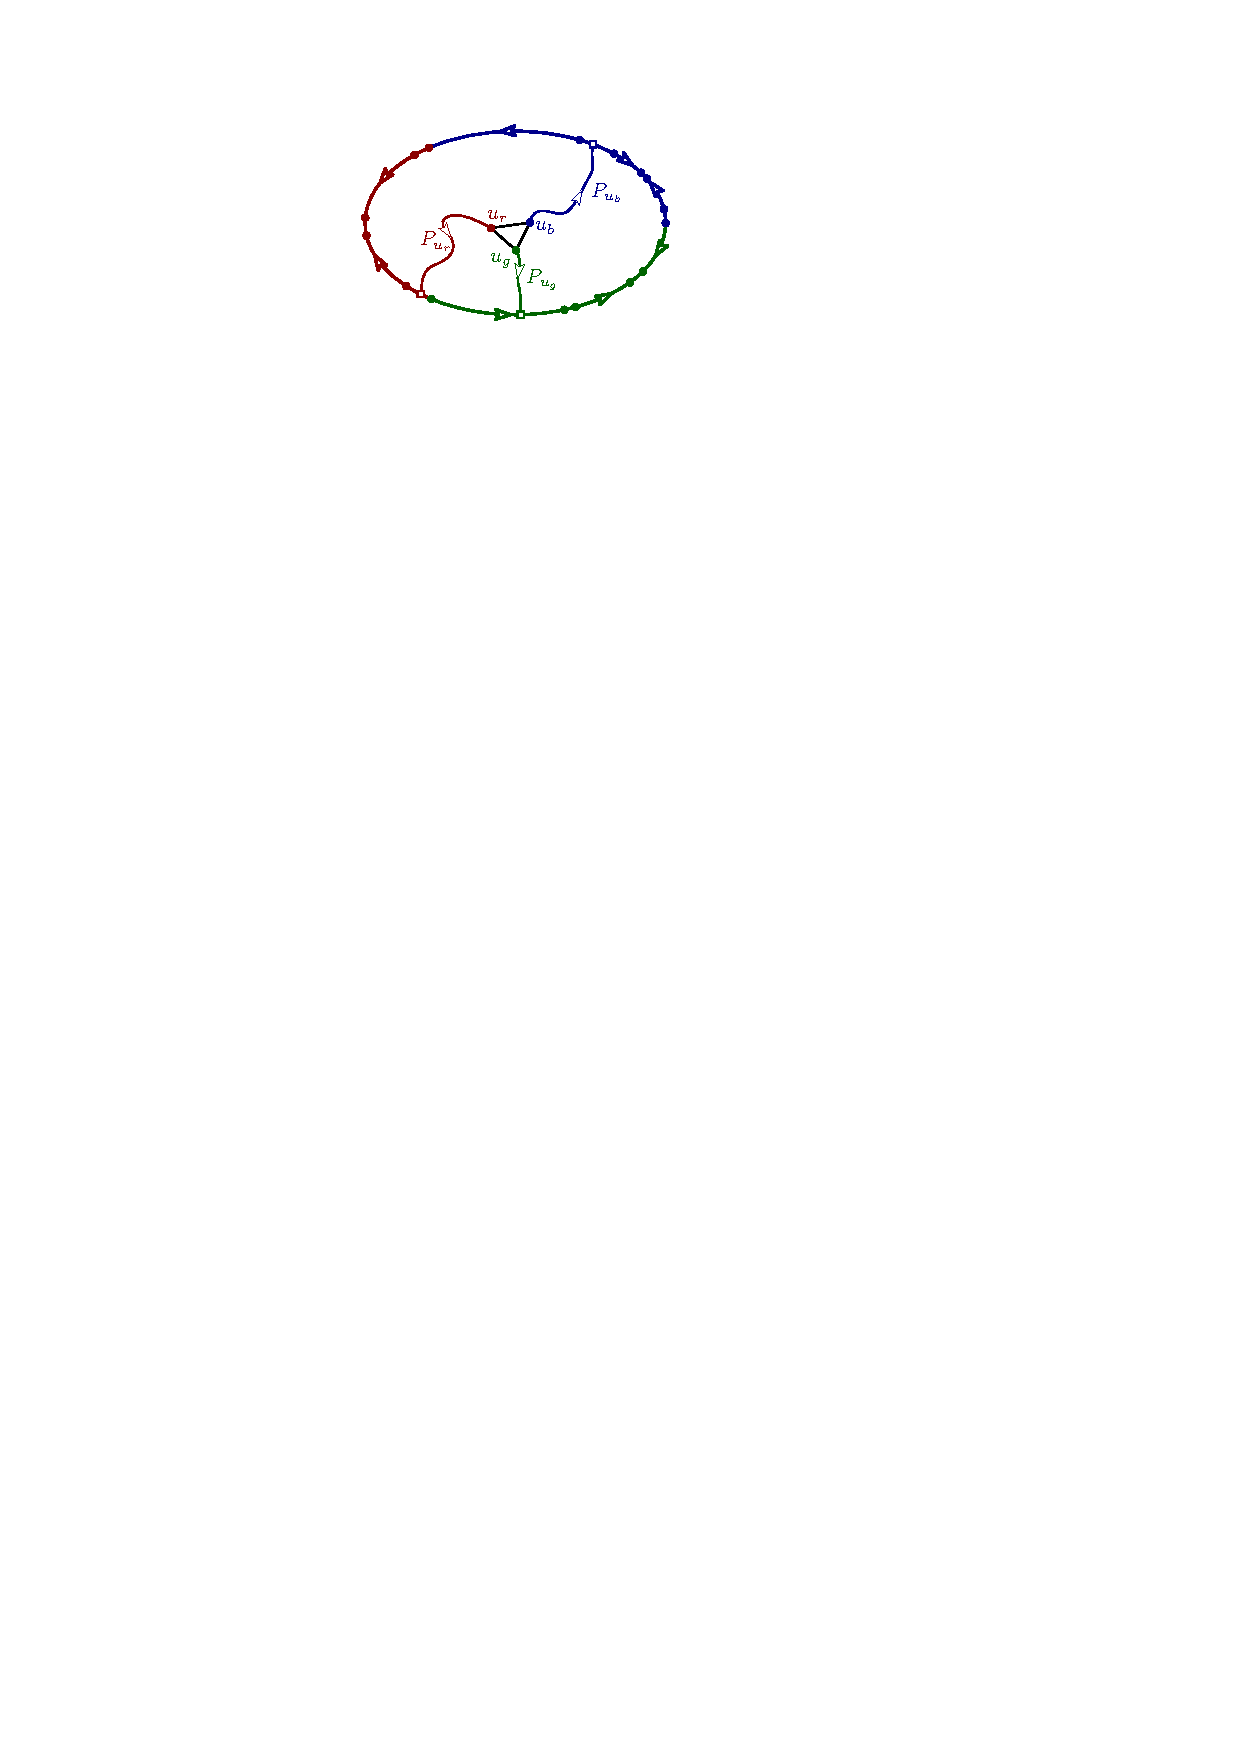
\includegraphics{sperner_simplified.pdf}
  \end{center}
  \caption{Finding a division that is not skewed.}\label{fig:division}
\end{figure}  

\paragraph{Many edges incident to a long path.} We assume now that the skeleton has $O(k)$ faces, each seeing at most $35$ segments. If we can show that the total branch degree (of the orginal solution $H$ without the artificial edges) is a constant in each face, then we can bound by $O(k)$ the total branch degree of the solution. We can observe, using the acyclicity of the edges inside the face, that we need to bound only the number of edges incident on the boundary.

Let $e$ be an edge inside the face incident to vertex $v$ of the boundary. We say that $e$ is \emph{essential} for demand $t_it_j$ if removing $e$ breaks every path from $t_i$ to $t_j$. Then we can define a path $P_e$ the following way: let us take any path $P$ from $t_i$ to $t_j$, and let $P_e$ be the subpath of $P$ starting from $e$ (which has to appear on $P$) to the first vertex on the boundary of $F$. Let us consider two edges $e_1$, $e_2$ starting from the same vertex $v$ of the boundary. Let us observe that $P_{e_1}$ and $P_{e_2}$ cannot intersect: then we could bypass e.g. $e_1$ by starting on $P_{e_2}$ and following it until intersection. By a similar argument, $P_{e_1}$ and $P_{e_2}$ cannot go to the same long segment: then one of $P_{e_1}$ and $P_{e_2}$ could be avoided by using the other path and part of the long segment. From these observations, it follows that the only way the boundary can have many edges incident to it is that if there are edges $e_1$, $\dots$, $e_s$ incident to distinct vertices of a long segment $S_1$, with paths $P_{1}$, $\dots$, $P_{s}$ going to distinct vertices of some other long segment $S_2$ (see Figure~\ref{fig:gridintro}).

\begin{figure}
  \begin{center}
    { \small \svg{0.6\linewidth}{findgridintro}}
  \end{center}
  \caption{Finding a grid.}\label{fig:gridintro}
\end{figure}


\paragraph{Finding a grid and a $t$-tough pair.} Now comes the point where we use the assumption that long segments are distant. In particular, this means that the ``middle path'' $P_{e_{s/2}}$ is long. The internal vertices of this path have no terminals (as all the terminals are on the skeleton), hence it is not possible that $d^+(v)=d^-(v)=1$ for any such internal vertex. Thus either there are many vertices on this path that have an edge leaving the path, or many vertices that have an edge entering the path. Assume without loss of generality the former, let $f_1$, $\dots$, $f_{s}$ be these edges. Again, each edge is essential for some demand, hence the path satisfiying the demand has a subpath $Q_{i}$ starting with $f_i$ and going to the boundary. We can observe again that these paths have to be disjoint. Therefore, we can obtain a grid-like structure in the region surrounded by $S_1$, $P_{s/2}$, $S_2$, and $P_s$, see the region highlighted by yellow in Figure~\ref{fig:gridintro}. (There are some other cases to consider, which we ignore here. For example, the paths $Q_i$ may go to $S_1$ or $S_2$.) This region has $s/2-1$ ``vertical'' paths $P_{s/2}$, $\dots$, $P_{s-1}$, intersected by the $s$ ``horizontal paths'' $Q_{1}$, $\dots$, $Q_s$.


We observe that if this grid has $t$ horizontal and vertical paths, then we can use it to discover a $t$-tough pair. Each edge $e_i$ is essential for some minimal demand; let $E_1$ be the set of these $t$ demands. Similarly, we define $E_2$ based on chosing a minimal demand for which $f_i$ is essential. Then we can carefully verify that $(E_1,E_2)$ is a $t$-\toughpair: if there is an edge in the demand graph that is not allowed, then a careful analysis shows that there is a way of bypassing some $e_i$ or $f_i$ in the grid, contradicting the fact that it is essential. This concludes the proof that if we have an upper bound on the size of the largest $t$-tough pair appearing in the graphs of class $\calD$, then we can bound the treewidth of the solution by $O(\sqrt{k})$.

 \paragraph{Cleaning.}
 To prove Theorem~\ref{thm:cleaning-intro}, we need to show that if arbitrary large $t$-tough-pairs appear in the graphs of $\calD$, then $\mathcal{C}_i\subseteq \calD$ for some $i\in[\kappa]$. The proof is a long combinatorial argument to show that we can find $t$-tough-pairs that are canonical in some sense, and then we use the assumption that $\calD$ is closed under identifying vertices to contract the vertices outside the $t$-\toughpair\ into a small constant number of well-behaved vertices.

 Suppose that there is a $t$-\toughpair $(E_1,E_2)$ in a digraph $D$.  The minimality of the edges in $E_1$ and the fact that they do not appear in directed cycles (as they are weakly independent to themselves) imply that for any two edges $x_iy_i, x_jy_j\in E_1$, at least one of the following holds:
 \begin{enumerate}
   \item exactly the edges $x_iy_j, x_jy_i$ appear between $\{x_i,y_i\}$ to $\{x_j,y_j\}$,
   \item there is no edge from $\{x_i,y_i\}$ to $\{x_j,y_j\}$, or
   \item there is no edge from $\{x_j,y_j\}$ to $\{x_i,y_i\}$.
   \end{enumerate}
   Let us consider a complete graph on $t$ vertices $w_1$, $\dots$, $w_t$, and for every $i<j$, color the edge $w_iw_j$ according to which of the three statements hold for the edges $x_iy_i$ and $x_jy_j$ (if more than one statement is true, we can choose arbitrarily). By Ramsey's Theorem, there is a large subset $E'_1\subseteq E_1$ where the same statement holds for any pair of edges. We can find a similar subset $E'_2\subseteq E_2$. We consider two main cases. The first case is when Statement 1 holds either in $E'_1$ or $E'_2$. Then what we have is a matching $x_iy_i$ of minimal edges that is part of a complete bipartite graph, that is, every $x_i$ is adjacent to every $y_j$ (but note that $x_iy_j$ does not have to be a minimal edge). The second case is where we have Statement 2 or 3 in both $E'_1$ and $E'_2$. Then we can reorder $E_1$ and $E_2$ to have a further ordering property: there is no edge from $\{x_i,y_i\}$ to $\{x_j,y_j\}$ for $j<i$. We handle the two cases separately. With further Ramsey arguments and case distinctions, we show that identifications can be used to find a $t'$-hard biclique pattern or a $t'$-hard matching pattern appearing in a graph in $\calD$, where $t'$ is some unbounded function of $t$. It follows that if arbitrarily large $t$-tough pairs appear in $\calD$, then $\calD$ is a superclass of some~$\mathcal{C}_i$.

%%% Local Variables:
%%% mode: latex
%%% TeX-master: "main"
%%% End:
